\section{Project Planning}

As proper planning tends to be one of the most important parts of working on any large-scale project, it was the first step of development.
Firstly, the main idea was put together, discussed with the team and refined so that the entire group was in agreement.
Next, we mapped out the high-level project requirements, planned the project management and development approach and split up roles.

At the start, we decided on 5 top-level requirements. These are as follows: \\
\textbf{REQ1.} Designed, Described and Implemented Search Engine Algorithm, optimized to find data relevant to user queries in tightly packed, dense technical text on external pages. \\
\textbf{REQ2.} Backend Service able to, at user request, crawl (relevant) subpages of a user given website and process them into a format defined for the Search Engine. \\
\textbf{REQ3.} Backend Functionality able to call the implemented Search Engine from REQ1 with a given user query, against the existing database from REQ2. \\
\textbf{REQ4.} Frontend Functionality with a search box and a result display page, capable of calling the Backend Functionality from REQ3 with an entered text query. \\
\textbf{REQ5.} Frontend Functionality allowing authorized and authenticated site visitors to add a new page to search, using the Backend Service from REQ2.\\ \\

These gave us a rough structure to work with. We further divided the requirements into sub-requirements (e.g. each portion of the search engine was its own requirement) to create a structure that would be easier to follow. The requirements structure was placed onto our GitHub project to be accessible by the team at any time. For more detail on the requirements, see our requirements document. \\
We followed up by dividing the tasks between each group member (for more detail, see the roles section). The project management plan was to utilise agile methodologies, with daily standups and 2-3 week long sprints. We kept track of people's progress through tickets using a GitHub project, notably making use of its kanban board view. There, the tickets could be organised by status, assignees, size, and planned due date.\\

\subsection{Timeline}
Most of the first semester was dedicated to research. Each member researched topics relevant to their tasks and summarised their findings to the group. After this, we begun working on the code. At first, each person worked on their own tasks, regularly reporting back to the team. Roughly halfway through the second semester we began putting the pieces together to make sure their interactions and interconnections work as expected. 
Towards the end of the semester we moved on to integrating the backend with the frontend and optimising the engine.\\
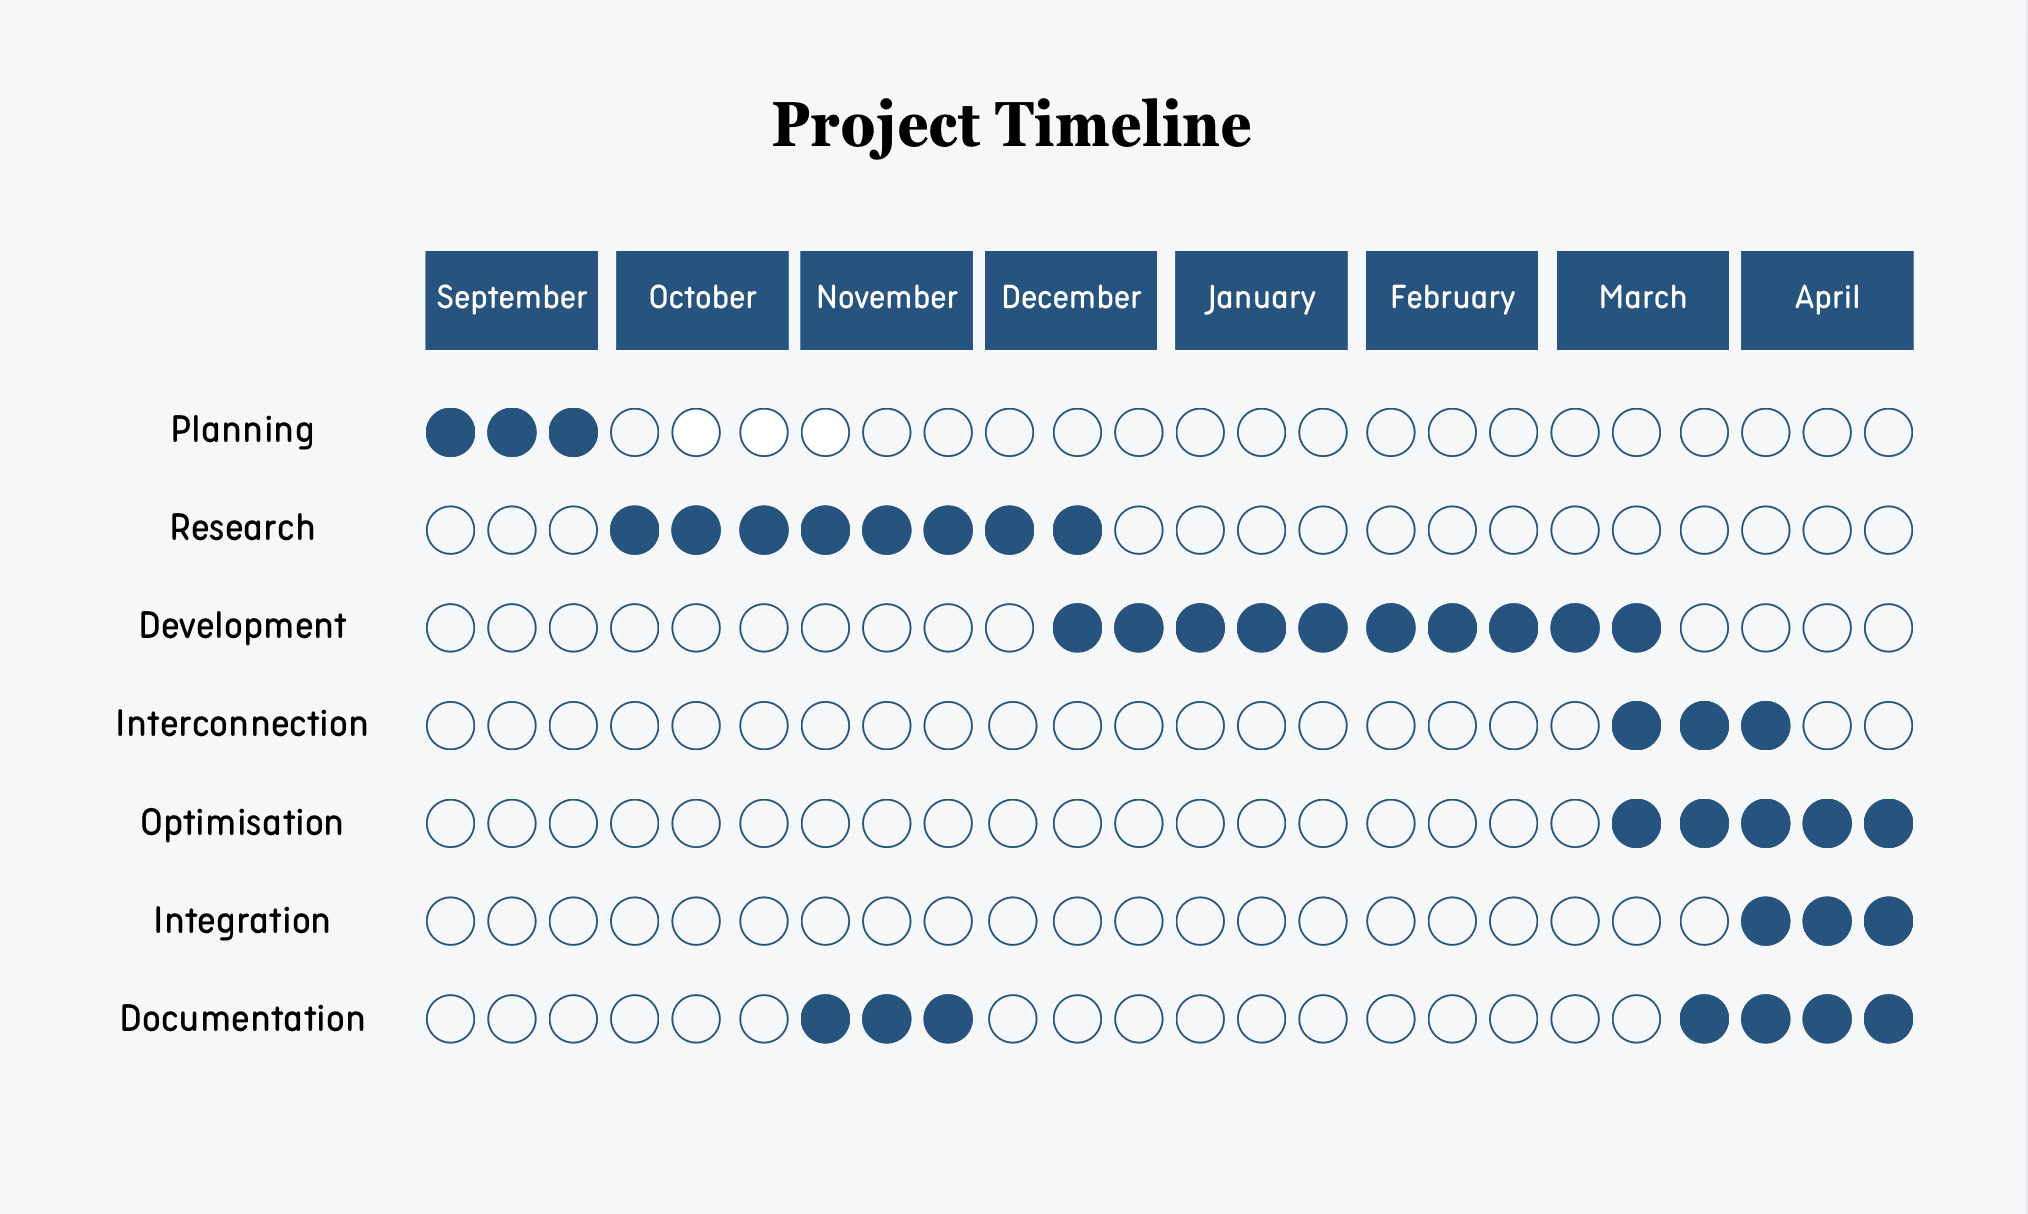
\includegraphics[width=\textwidth,keepaspectratio]{timeline.png}\\
